% {{{
\documentclass[12pt]{article}
\usepackage[tmargin=0.75in,bmargin=0.75in,lmargin=0.9in,rmargin=0.9in]{geometry}

\usepackage{amsmath}
\include{latexsym}
\include{amssymb}
\usepackage{enumitem}
\usepackage[symbol, hang]{footmisc}
\usepackage{indentfirst}
\usepackage{amssymb}
\usepackage{graphicx,psfrag}

\def\F{\mathcal{F}}
\def\M{\mathcal{M}}
\def\dimspec{\mathfrak{D}}
\def\htop{h_{top}}
\def\trans{\mathcal{T}}
\def\G{\mathcal{G}}
\newcommand{\Z}{\mathbb{Z}}
\pagenumbering{gobble}
\def\O{\mathcal{O}}

\newcommand\NoIndent[1]{%
  \begingroup
  \par
  \parshape0
  #1\par
  \endgroup
}
% }}}

% Title {{{
\begin{document}

\begin{center}
{\large \bf CompMethods }   \\ \large pset6 \\ Ephraim Sutherland
\end{center}
% }}}

\subsection*{Problems}

\begin{enumerate}

\item 
	\begin{center}
		\textbf{a}\par\medskip
		\includegraphics[width=0.9\linewidth]{Q1fig1.png}
	\end{center}
At $N = 5$, maxmimum difference for cubic spline is $0.10066905152426586$ and mean difference is $0.049741733407626165$
\\At $N = 5$, maxmimum difference for linear interpolation is $0.21050926086358024$ and mean difference is $0.13593608051703687$
\\At $N = 11$, maxmimum difference for cubic spline is $0.009113248124472395$ and mean difference is $0.001583183096282803$
\\At $N = 11$, maxmimum difference for linear interpolation is $0.048912330599002796$ and mean difference is $0.02097995955150908$
\\At $N = 21$, maxmimum difference for cubic spline is $0.0011833085882222982$ and mean difference is $0.00010538718916869369$
\\At $N = 21$, maxmimum difference for linear interpolation is $0.012139714245095079$ and mean difference is $0.00522110569007282$

\item
	\begin{center}
		\textbf{a}\par\medskip
		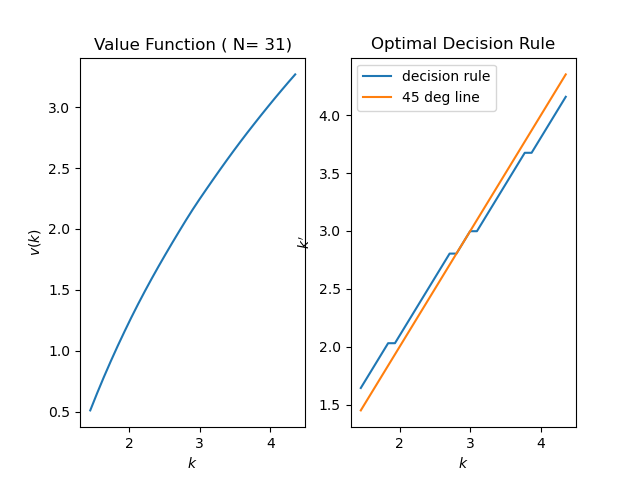
\includegraphics[width=0.8\linewidth]{Q2fig1.png}
		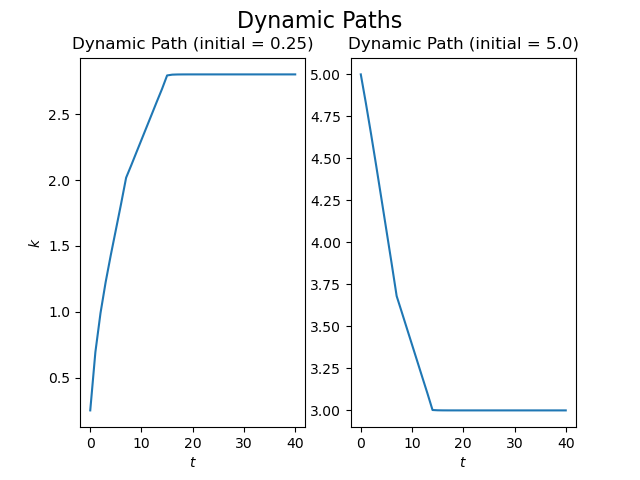
\includegraphics[width=0.8\linewidth]{Q2fig2.png}
	\end{center}

\item 
		
	\begin{center}
		\textbf{a}\par\medskip
		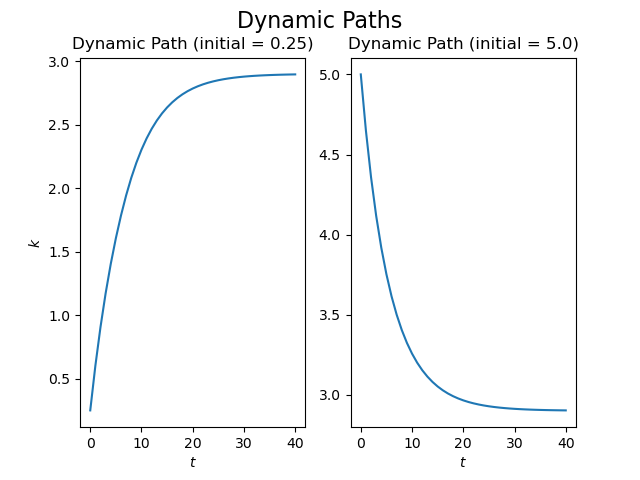
\includegraphics[width=0.8\linewidth]{Q3DynamicPaths.png}
		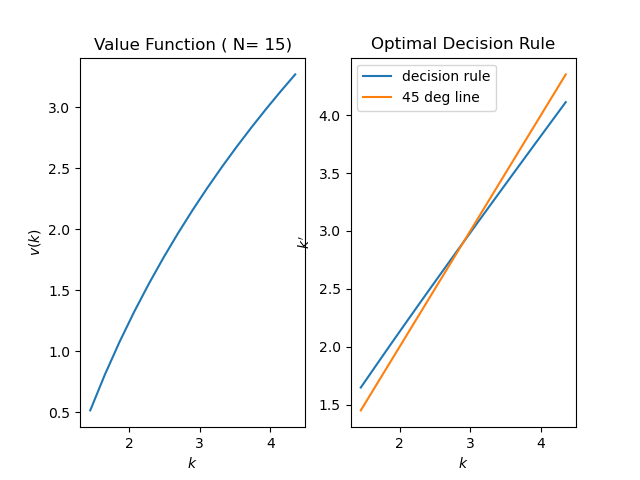
\includegraphics[width=0.8\linewidth]{fig1.png}
	\end{center}
\end{enumerate} 

\end{document}


